\section{Analyse}
\label{sec:Analysis}


\subsection{Netzwerkeigenschaften}
\label{sec:overview-numbers}
Als erstes soll die Art des Netzwerkes analysiert werden. Der Begriff \guillemotleft Hub\guillemotright wird sehr
häufig im Zusammenhang mit Luftfahrt und Flughäfen verwendet.
Deshalb wird auch erwartet, dass das Netzwerk ein natürliches bzw. skalenfreies Netzwerk bildet.
Zufällige Netzwerke haben eine gleichmässige Gradverteilung während die Verteilung bei natürlichen Netzwerken einem
Potenzgesetz folgt.
Das Histogramm der Knotengrade deutet sehr stark auf eine exponentielle Verteilung hin (siehe Abb. \ref{fig:degreeHistogram}).

\begin{figure}
    \centering
    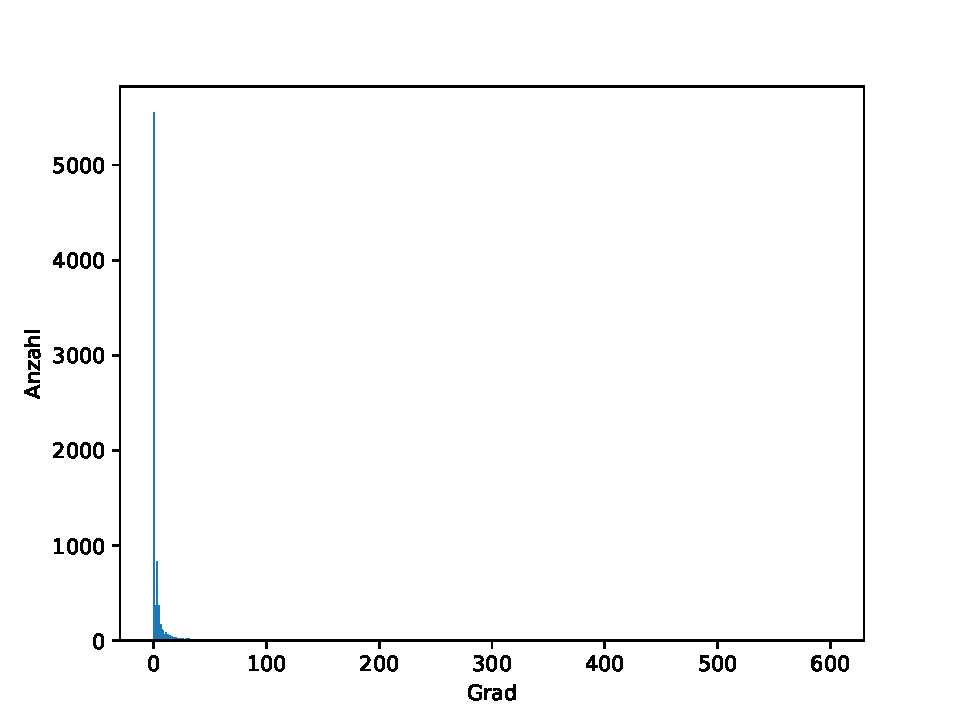
\includegraphics[width=0.75\linewidth]{images/degree-histogram.pdf}
    \caption{Caption}
    \label{fig:degreeHistogram}
\end{figure}

\subsection{Beschaffenheit}

\subsubsection{Übersicht}

Die Daten basieren auf dem Datensatz für die Flughäfen vom 8. Oktober 2018 sowie Flugverbindungen vom 9. November 2018.


\begin{tabular}{l|l}
    Durchschnittler Grad $ \langle k\rangle $ & 38.215\\ \hline
    Zweites Moment $ \langle k^{2}\rangle $ & 35676.88 \\ \hline
    Exponent $ \gamma $ & 2.24 \\ \hline
\end{tabular}

\subsubsection{Annäherung \gamma-Exponent}
Gemäss des Algorithmus in Network Science \footnote{} soll der Gamma-Exponent für das Flugroutennetzwerk angenähert werden.

Zur Schätzung des $ \gamma$- Exponenten wird die Maximum Likelihood Methode wie in \cite{barabasi-network-science} und näher
in \cite{clauset-power-law-distribution} beschrieben.

$$ \gamma = 1 + N\Bigg[\sum_{i=1}^{N}ln \frac{k_{i}}{K_{min} - \frac{1}{2}}\Bigg]^{-1} $$


\subsubsection{Berechnung }


\section{Erste Forschungsfragen}
\label{sub:scientific-questions}

\begin{enumerate}
    \item Welches sind die wichtigsten Flughäfen?
    \item Wie korreliert die Erdumrundungszeit mit der Robustheit des Flugnetzwerkes?
    \item Wie ist die Beschaffenheit des globalen Flughafennetzwerkes im Bezug auf die Robustheit?
\end{enumerate}

\subsection{Ausarbeitung}
\label{subsec:scientific-question-analysis}

\subsubsection{Welches sind die wichtigsten Flughäfen?}
Begründung: Wichtig für die Funktionstüchtigkeit des Netzwerks

\subsubsection{Wie ist die Beschaffenheit des globalen Flughafennetzwerkes im Bezug auf die Robustheit?}
Begründung: Im Flugnetz finden täglich bis zu 200000 Flugbewegungen statt \footnote{http://www.reisereporter.de/artikel/4533-rekord-tag-luftfahrtgeschichte-flugzeuge-und-fluege-pro-tag-weltweit-flug-tracker-flightradar-misst-verkehrsreichsten-tag}.
Für diese enorme Zahl finden erstaunlich wenige Störungen und Ausfälle statt.
Aber wie gut ist das Netzwerk aufgebaut?
Wieviele Flughäfen müssten ausfallen, damit das Gesamtnetz in einzelne isolierte Unternetze zerfällt und damit der weltweite Luftverkehr zum erliegen kommt?
Robustheit, relevanz? Heisst: Wie lange hängen alle noch aktiven Flughäfen zusammen?

Random Failuers: f_c = 1 - \frac{1}{\frac{\langle k^{2}\rangle}{\langle k\rangle} - 1} = 0.775533

\subsubsection{Welches ist der Zeitgünstigste Weg, um von Zürich nach Zürich einmal um die Welt zu fliegen?}
Begründung: Aviatik hat jeden Punkt auf der Erde in wenigen Stunden erreichbar gemacht. Aber wie lange dauert eine komplette Erdumrundung konkret?

\section{Literatur-Recherche}
\label{subsec:literature-research}

Robustheit

\guillemotleft Worldwide aviation network vulnerability analysis: a complex network approach \guillemotright
https://link-springer-com.proxy2.biblio.supsi.ch/content/pdf/10.1007%2Fs40844-015-0025-y.pdf

Als besseres Mass für die Robustheit gilt die die Auswirkung auf die Effizienz, wenn bestimmte Flughäfen aussteigen.


\subsection{Verspätungen}
Mobilität per Flugzeug wächst seit Beginn der Luftfahrt.
In einem kürzlich erschienenen Artikel spricht die NZZ gar von einem jährlichen Wachstum der Anzahl Flüge von 4\%\footnote{https://www.nzz.ch/wirtschaft/wieso-in-europa-viel-zu-viele-fluege-verspaetet-sind-ld.1410842}.
Im selben Artikel werden die Auswirkungen dieses immer dichter werdenden Verbindungsnetzwerks dargelegt: Häufigere und längere Verspätungen.
Ursachen für Verspätungen sind z.B. Streiks, Wetterbedingungen, Verkehrsüberlastungen, aber auch ineffiziente Arbeitsabläufe während des sog. \guillemotleft Turnarounds\guillemotright,
die Zeit, während der das Flugzeug geparkt ist und entladen, betankt und wieder beladen bzw. für den nächsten Flug vorbereitet wird.

In diesem Abschnitt soll in Anlehnung an zwei relevanten wissenschaftlichen Artikeln ein Modell erarbeitet werden,
um die \guillemotleft Anfälligkeit\guillemotright des europäischen Flugnetzwerkes auf sich kumulierende Verspätungen zu untersuchen.

Dabei soll versucht werden, folgende zwei Fragestellungen zu beantworten:

\begin{enumeration}
    \item Wie verhält sich ein bestimmter Verspätungs-Grenzwert, ab dem das System komplett zum erliegen kommt?
    \item Wie verhält sich die Netzwerk-Gesamtverspätung an einem Tag in Abhängigkeit der Netzwerkbeschaffenheit?
\end{enumeration}

\subsubsection{Modell}
\label{subsubsec:model}

Zunächst muss ein Modell erstellt werden, welches sich zur Simulation einer zeitlichen Entwicklung der Verspätungen eignet.
Q. H. Anh Tran und Akira Namatame \cite{anh-tran-worldwide-aviation-network} analysieren in ihrem Artikel das Verhalten
der Effizienz des weltweiten Flugnetzwerkes bei Totalausfall einzelner Flughäfen (Streiks, Kriminalfälle, …) anhand eines vereinfachten und ungerichteten Graphs.
Sie beschreiben zunächst das Netzwerk anhand einer NxN-Matrix, in der jede Verbindung zwischen Flughafen $ i $ und Flughafen $ j $
mit dem Gewicht $ w_{ij} $ eingetragen ist.
Das Gewicht ist die Summe aller Verbindungen zwischen den beiden Flughäfen dar.
Finden beispielsweise vier Flüge von Zürich nach London am Tag statt, so beträgt das Gewicht $ w_{Zuerich London}$ 4.
Im Weiteren wird jedem Flughafen eine Initiallast $L_{i}$ sowie eine Maximalkapazität $ C_{i} = \alpha L_{i}$ zugeordnet.
Die Last errechnet sich aus der Summe aller \guillemotleft effizientesten\guillemotright Pfade, die über den Flughafen $i$ führen.
Dies entspricht ähnlich der \guillemotleft Betweenness Centrality\guillemotright einer Art \guillemotleft Effizienzzentralität\guillemotright.
Im Artikel wird die Nähe zwischen zwei Flughäfen nicht nach dem geografischen Merkmal definiert, sondern nach dem Umkehrwert der Anzahl Direktflügen,
die zwischen den Flughäfen stattfinden ($ p_{ij} = \frac{1}{w_{ij}} $).
Als Distanz zwischen zwei entfernten Flughäfen gilt: $ d_{ij} = \sum_{n=0}^{^k-1}\frac{1}{w_{i_{n}i_{n + 1}}}$.
Die Effizienz ist dann schliesslich: $ e_{ij} = \frac{1}{d_{ij}}$.

Für die vorliegenden Fragestellungen soll das Konzept der Effizienz aus dem Modell von\cite{anh-tran-worldwide-aviation-network} als Grundlage herangezogen werden.
Für die weiteren Details eignet sich aber das Model von Fleurquin und Ramasco besser\cite{fleurquin-ramasco}.
Grundsätzlich funktioniert die Simulation so, dass durch diverse Ereignisse initial Verspätungen entstehen, die durch die
Flugverbindungen an die Zielflughäfen weitergericht werden.
Ein Flughafen wird somit mit Verspätungszeit \guillemotleft aufgeladen\guillemotright und gibt diese Zeit teilweise an die weiteren Abflüge weiter.

Dazu wird das Modell wie folgt aufgebaut und simuliert:

\begin{itemize}
    \item Vorbereitend wird für sämtliche Flughäfen die Maximalkapazität berechnet. Ähnlich \cite{anh-tran-worldwide-aviation-network} wird davon ausgegangen, dass das Netzwerk im Normalzustand nahe an der Maximalkapazität arbeitet. Als Grundlage wird daher die maximale Anzahl Flugbewegungen (Abflüge und Ankünfte), die ein Flughafen pro Stunde abfertigt verwendet. Die Maximalkapazität wird mit dem Faktor $\alpha = 1.2$ berechnet.
    \item Die Simulation beginnt um Mitternacht, 0:00 Uhr. Ein Zeitschritt beträgt eine Minute. Für eine komplette Simulation (ein Tag) werden also 1440 Zustände berechnet.
    \item Für jeden Zeitschritt werden sämtliche zu diesem Zeitpunkt startenden Flüge betrachtet. Starten von einem bestimmten Flughafen mehr Flüge als seine Maximalkapazität erlaubt, wird exponentiell zum Mehraufwand eine kapazitätsbedingte Verspätung generiert.
    \item Wurden dem Abflughafen bereits Verspätungen von ankommenden Flügen deponiert, so werden diejenigen Verspätungen an die Abflüge weitergereicht, deren Entstehungszeitpunkt addiert zum Betrag der Verspätung sowie der Bodenzeit und etwaiger Kapazitätsverspätung den jeweiligen Abflugzeitpunkt übersteigen. Verspätungen, die weit vor einem Abflug entstanden sind, haben somit keinen Einfluss auf den effektiven Abflugzeitpunkt. Unter allen in Frage kommenden Verspätungen wird anschlissend diejenige zu einem gewissen Anteil an die Flugzeit als Verspätung addiert, die zum Abflugzeitpunkt die grösste Überlappung erzeugt.
    \item Für jeden Flug wird eine En-Route-Verspätung von -15 bis +15 Minuten generiert. Damit sollen einerseits Zeitgewinne durch Abkürzungen und höhere Leistung und andererseits Verspätungen durch Wetterbedingungen o.ä. abgebildet werden.
    \item Flughäfen \guillemotleft erholen\guillemotright sich linear von den Verspätungen. Eine Stunde angesammelter Verspätung wird in einem Zeitraum von vier Stunden komplett abgebaut. Dies widerspiegelt die Massnahmen der Flughäfen, um Verspätungen entgegenzuwirken. Etwa durch effizientere Arbeit oder Bevorzugung gewisser verspäteter Flüge auf Kosten anderer Verbindungen.
    \item Hat ein Flug Verspätung, so wird seine Ankunftszeit angepasst. Dies hat wiederum Auswirkungen auf die Last bzw. mögliche Kapazitätsengpässe beim Zielflughafen.
    \item Als durchschnittliche \guillemotleft Turn around\guillemotright Zeit werden 45 Minuten berechnet.
    \item Der Anteil an Passagieren, der auf einen Anschlussflug umsteigt, wird mit 40\% berechnet.
\end{itemize}

Eine Validierung und Präzisierung dieses Modells würde den zeitlichen Umfang der Arbeit übertreffen.
Die Berechnungen des Modells dienen somit lediglich zur qualitativen Analyse des Netzwerks.

Das Resultat eines ersten Durchlaufs der Simulation ist in Abb. \ref{fig:first-simulation-run} ersichtlich.
Darin ist ein starker Anstieg der gesamteuropäischen Verspätung hin zur Mittagszeit zu beobachten, der sich nach der
Mittagszeit genau so schnell wieder abbaut.
Eine Visualisierung der Anzahl Abflüge und Ankünfte (als Summe Anzahl Flugbewegungen) innerhalb Europas macht den
Hintergrund dieser Verspätungsentwicklung deutlich (siehe Abb. \ref{fig:arr-dep-europe}).
Interessanterweise hat eine Erhöhung des Kapazitätsfaktors keinerlei Auswirkung auf die Verspätungsentwicklung.
In zweiter Hinsicht liegt dies jedoch auf der Hand, da die Hauptursache der Verspätungen offensichtlich darin liegt, dass
verspätete Flüge abgewartet werden müssen.
Dies ist auch der Fall, wenn der Flughafen doppelt so viele Landungen zulassen würde.
Deswegen holt ein Flug seine Verspätung allerdings nicht auf (allenfalls minim durch eine frühere Landung ohne Warteschlaufe).

Umgekehrt stellt sich nun die Frage, wie sich die entwicklung der Verspätung in Abhängigkeit der Netzwerkbeschaffenheit ändert.
Im zuvor erwähnten NZZ-Artikel wird von einer Wachstumsrate der Flüge von jährlich 4\% ausgegangen.
In einer weiteren Simulation wird das empirische Netzwerk einem entsprechenden Wachstum für fünf, zehn, 15 beziehungsweise 20 Jahre ausgesetzt.
Das Netzwerk wird dabei jeweils um die Zeit von 5:00 Uhr morgens bis 20:00 Uhr abends mit dem Wachstum entsprechenden zusätzlichen Verbindungen ausgestattet.

5:
112437
136796
27998.155082216195

10:
112437
166434
max 33819.02327609417

15:
112437
202491
max 40147.514825236954


20:
112437
246362
max 48335.76


Wie verhält sich die Verspätungsentwicklung in einem zufälligen Netzwerk?
Zu diesem Zweck wird das empirische Flugnetzwerk in ein zufälliges Netzwerk transformiert.
Dabei werden die Flughäfen als Knoten beibehalten, die Verbindungen werden allerdings zufällig zwischen allen
Knoten verteilt.
Abbildung \ref{fig:total-delay-random} zeigt eindrücklich den Unterschied in der Entwicklung der Verspätungen.
Das Zufallsnetzwerk scheint die Weiterverbreitung der Verspätungen besser zu absorbieren als das natürliche Netzwerk.
Dies könnte damit erklärt werden, dass das Potenzial von \guillemotleft Flaschenhälsen\guillemotright in einem
zufälligen Netzwerk weitaus geringer ist als in skalenfreien Netzwerken.
Sind Hubs vorhanden, so ist die Wahrscheinlichkeit gross, dass viele Flüge zur selben Zeit an einem Flughafen ankommen
und möglicherweise einen starken Anstieg der Gesamtverspätung mit sich bringen.
Gleichzeitig wird diese Verspätung mit den Anschlussflügen an sehr viele weitere Flughäfen verteilt.
Anders im Zufallsnetzwerk: Zwar ist die Summe aller Verspätungen der europäischen Flughäfen anfangs grösser, weil
die Verspätung von mehr Flughäfen einzeln gezählt wird als beim natürlichen Netzwerk.
Später wächst die Verspätung allerdings sehr wenig, da die Verspätungen auf mehr Flughäfen verteilt werden können und
weniger Anschlussflüge von einem verspäteten Flug abhängig sind.

\begin{figure}
    \centering
    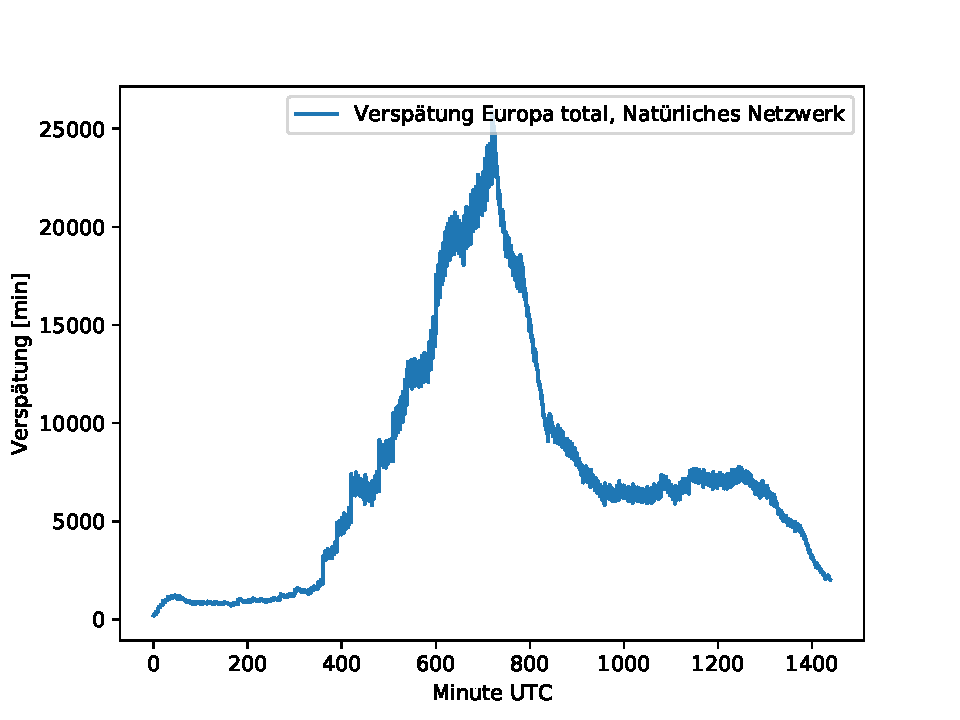
\includegraphics[width=0.75\linewidth]{images/total-delay-first-simulation-run.pdf}
    \caption{Simulation der gesamteuropäischen Verspätung}
    \label{fig:first-simulation-run}
\end{figure}

\begin{figure}
    \centering
    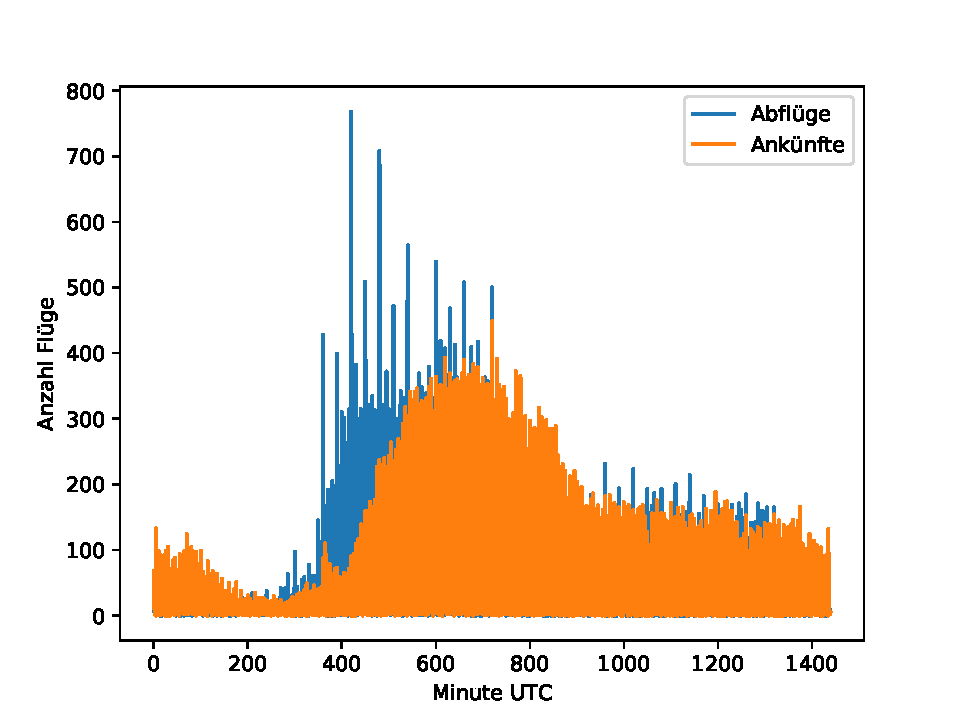
\includegraphics[width=0.75\linewidth]{images/arr_dep_europe.pdf}
    \caption{Anzahl Flugbewegungen}
    \label{fig:arr-dep-europe}
\end{figure}

\begin{figure}
    \centering
    \subfigure{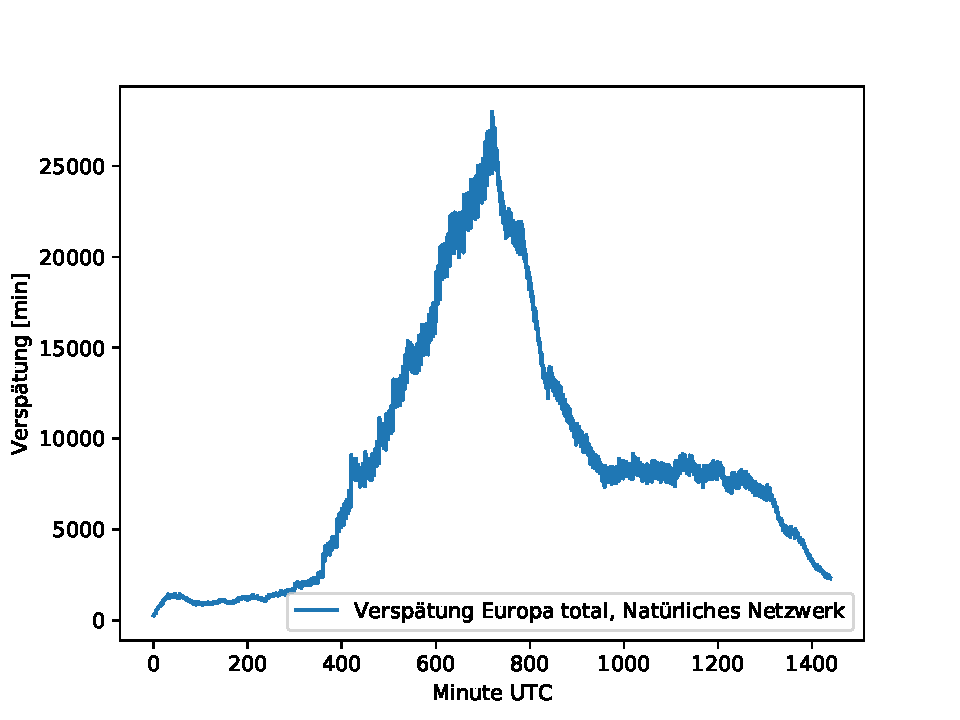
\includegraphics[width=0.45\linewidth]{images/total_delay_5yrs.pdf}}
    \subfigure{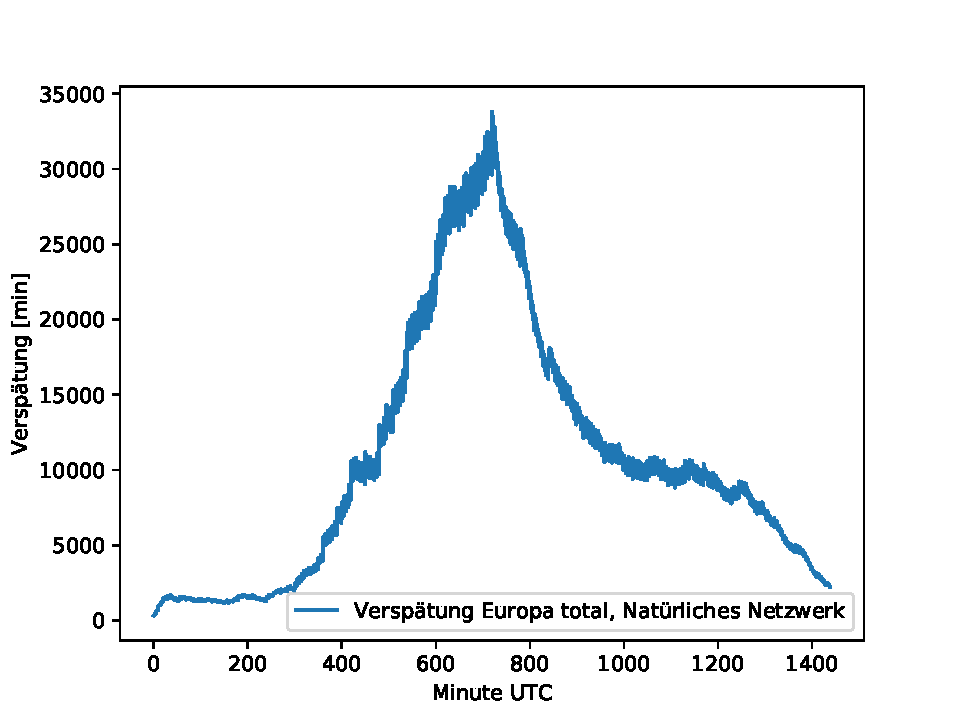
\includegraphics[width=0.45\linewidth]{images/total_delay_10yrs.pdf}}
    \subfigure{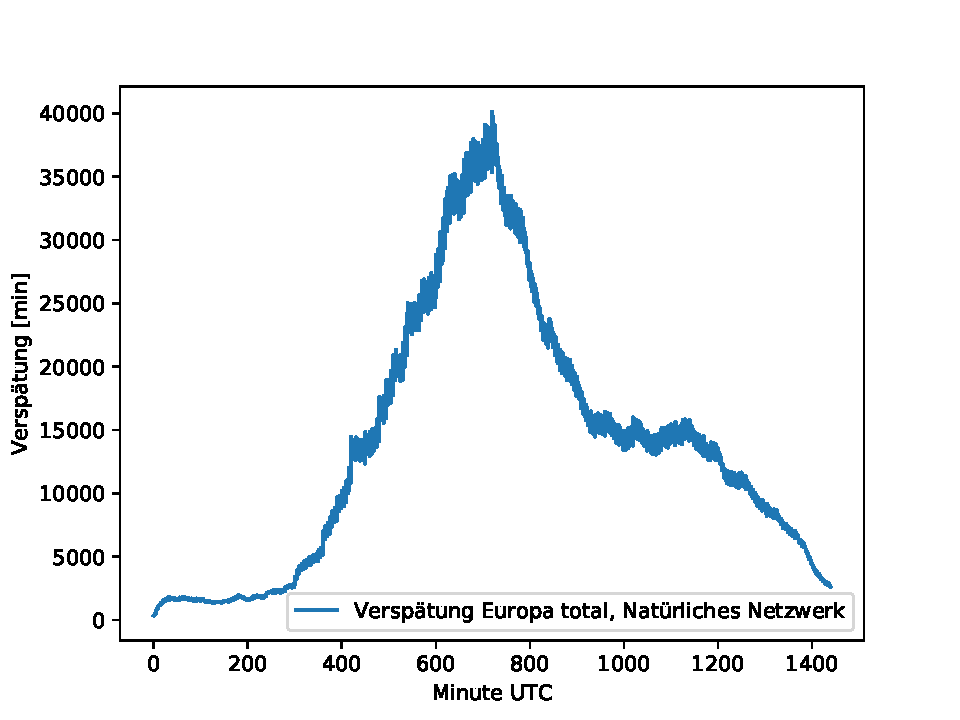
\includegraphics[width=0.45\linewidth]{images/total_delay_15yrs.pdf}}
    \subfigure{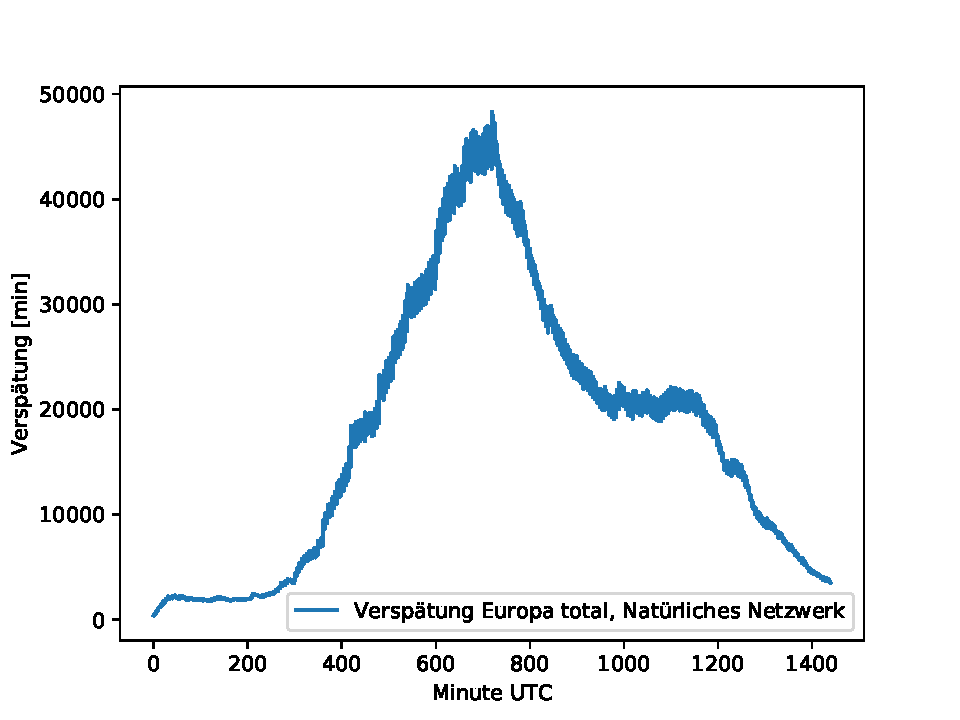
\includegraphics[width=0.45\linewidth]{images/total_delay_20yrs.pdf}}
\end{figure}

\begin{figure}
    \centering
    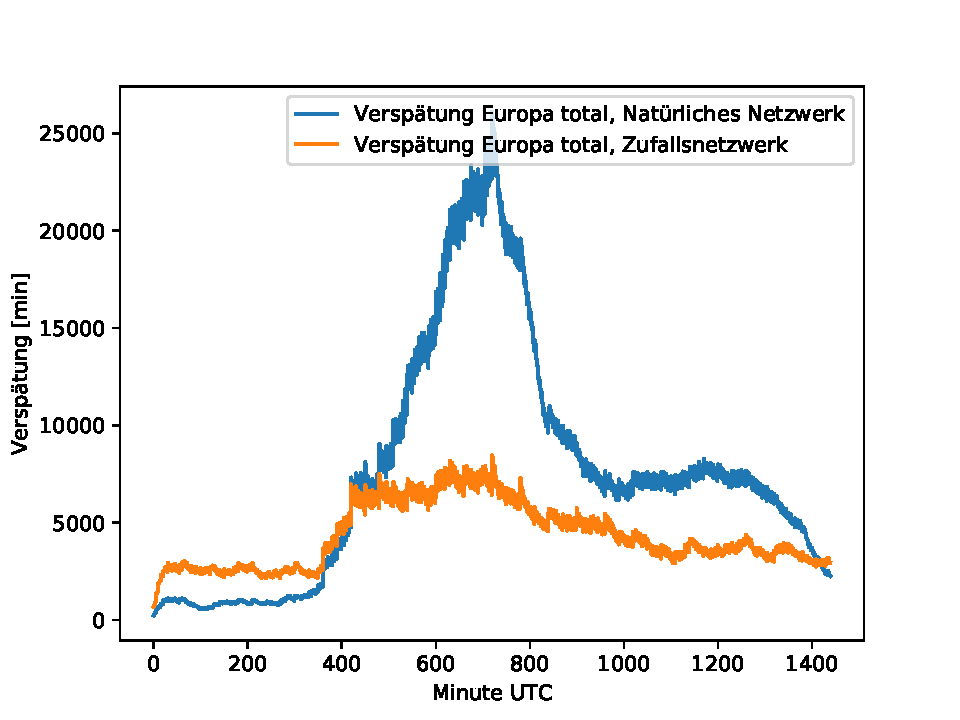
\includegraphics[width=0.75\linewidth]{images/total_delay_random.pdf}
    \caption{Simulation der gesamteuropäischen Verspätung mit Zufallsnetzwerk}
    \label{fig:total-delay-random}
\end{figure}

Natürlich widerspiegelt ein zufälliges Netzwerk die Realität in keinster Weise, aber es liefert zumindest Anhaltspunkte,
wie die zukünftige Entwicklung des natürlichen Netzwerkes optimal gestaltet werden könnte.

In diesem Zusammenhang kann folgende weitere Hypothese aufgestellt werden: \guillemotleft Die Gesamtverspätung des
europäischen Flugnetzwerkes nimmt weniger zu, wenn beim Ausbau des Netzwerks vor allem Direktverbindungen
bevorzugt werden, als wenn Verbindungen gemäss der bereits vorhandenen Hub-Struktur angehäuft werden.\guillemotright.

Um dies zu untersuchen, soll die Simulation auf zwei Arten angepasst werden:
\begin{enumerate}
    \item Das Wachstum des Netzwerks über 10 Jahre bevorzugt Flughafenpaare, zwischen denen bereits eine starke Verbindung (sprich viele tägliche Verbindungen) besteht.
    \item Das Wachstum des Netzwerks über 10 Jahre bevorzugt Flughafenpaare, zwischen denen bereits eine starke Verbindung besteht, stellt stattdessen jedoch Direktverbindungen zwischen einem der beiden Flughäfen und einem direkten Nachbarn des anderen Flughafen her.
\end{enumerate}

Analog zum Barabási-Albert Modell wird die Verbindungswahrscheinlichkeit für Fall 1 wie folgt beschrieben:

\begin{equation}
    \label{eq:growth-model-1}
    \prod (k_{ij}) = p\frac{1}{N} + (1-p)\frac{w_{ij}}{\sum_{z}w_{iz}}
\end{equation}

Ein bestehender Flughafen $i$ stellt also während des Wachstums zunächst zu jedem anderen Flughafen $j$ mit der Wahrscheinlichkeit
$p \frac{1}{N}$ eine Verbindung her.
Existieren zwischen den Flughäfen $i$ und $j$ hingegen bereits Verbindungen, so steigt die Verbindungswahrscheinlichkeit in Abhängigkeit
der Anzahl $w_{ij}$ dieser bereits bestehenden Verbindungen im Verhältnis zu allen bereits bestehenden Verbindungen ausgehend von Flughafen $i$ (siehe Abb. \ref{fig:pref-attach-hubs}).
Dies soll die Realität beschreiben, wo bereits beliebte Flugrouten durch die steigende Nachfrage in der Kapazität (sprich Anzahl Flüge pro Tag)
ausgebaut werden.

Für den zweiten Fall dient Gleichung \ref{eq:growth-model-1} als Basis, allerdings mit der Änderung, dass bestehende Direktverbindungen \textit{nicht} weiter
ausgebaut werden sollen.
Stattdessen sollen neue Verbindungen zu den Nachbarn dieser bestehenden Direktverbindungen hergestellt werden, wenn zu diesen Nachbarn noch keine
oder nur wenige Direktverbindungen bestehen (siehe Abb. \ref{fig:pref-attach-neighbors}).

\begin{equation}
    \label{eq:growth-model-2}
    \prod (k_{in}) = p\frac{1}{N} + w_{n}\Bigg[ (1-p)\frac{1}{1 + w_{in}^{2}}\frac{w_{ij}}{\sum_{z}w_{iz}} \Bigg], w_{n} = \begin{cases}1,& \text{falls } w_{jn}\geq 1\\ 0, & \text{andernfalls}
    \end{cases}
\end{equation}

Gleichung \ref{eq:growth-model-2} erhöht die Verbindungswahrscheinlichkeit nur dann, wenn zwischen den Hub-Flughafen $j$ und dessen Nachbar $n$ bereits mindestens eine Verbindung besteht.
Ist dies nicht der Fall, ist eine Direktverbindung von $i$ nach $n$ nicht sinnvoll, weil Passagiere bereits heute nicht von $i$ nach $n$ reisen.
Die Wahrscheinlichkeit, dass $i$ eine Verbindung nach $n$ herstellt unterliegt dann also einem gleichmässigen Zufall.

Besteht allerdings bereits mindestens eine Verbindung zwischen Hub und Nachbar, so ist es umso wahrscheinlicher, dass eine Direktverbindung von $i$ nach $n$ aufgebaut wird,
je weniger Direktverbindungen zwischen diesen Flughäfen bereits bestehen ($ \frac{1}{1 + w_{in}^{2}}$).

Dies soll das Bestreben des Wachstums widerspiegeln, Lasten von Hubs abzuwenden und stattdessen auf noch wenig entwickelte Direktrouten zu verteilen.





\begin{figure}
    \centering
    \subfigure[\label{fig:pref-attach-hubs}]{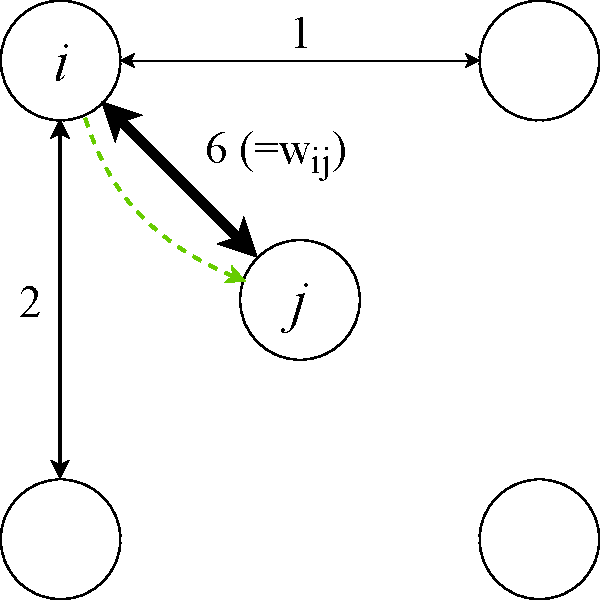
\includegraphics[width=0.30\linewidth]{images/growth-model-1.pdf}} \hspace{4em}
    \subfigure[\label{fig:pref-attach-neighbors}]{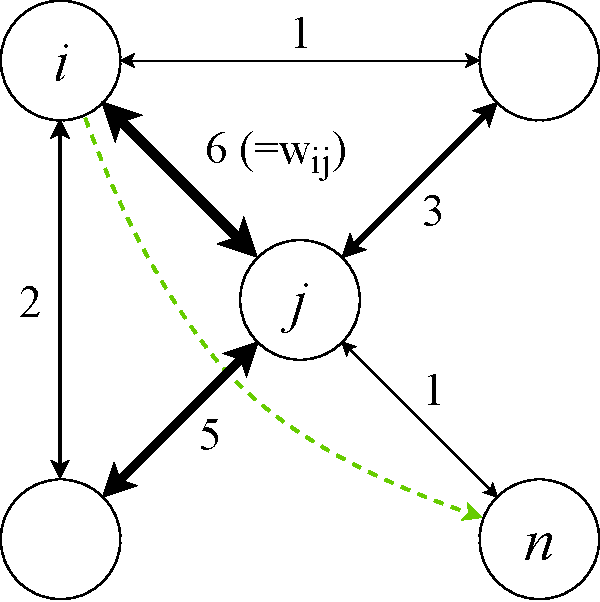
\includegraphics[width=0.30\linewidth]{images/growth-model-2.pdf}}
    \label{fig:pref-attach}
    \caption{Bevorzugung von Hubs (a) sowie von Nachbarn von Hubs (b)}
\end{figure}



\subsubsection{Wie verhält sich die Netzwerk-Gesamtverspätung an einem Tag in Abhängigkeit der Netzwerkbeschaffenheit?}
\label{subsubsec:question-1}

Konkret formuliert lautet die Frage: \guillemotleft Entwickelt sich die Gesamtverspätung anders in einem Zufallsnetzwerk als
in einem natürlichen Netzwerk? \guillemotright bzw. \guillemotleft Wäre eine gleichmässigere Verbindungsverteilung
vorteilhafter für die Anfälligkeit für Verspätungskaskaden? \guillemotright



\subsubsection{Wie verhält sich ein bestimmter Verspätungs-Grenzwert, ab dem das System komplett zum erliegen kommt?}

Ab wann gilt, dass das komplette System zum erliegen kommt?



\guillemotleft Systemic delay propagation in the US airport network \guillemotright
https://www.nature.com/articles/srep01159
https://www.nzz.ch/wirtschaft/wieso-in-europa-viel-zu-viele-fluege-verspaetet-sind-ld.1410842
http://www.airliners.de/flugzeug-stehzeug-wie-bodenzeit-jets-jenny-jetstream-50/34225
https://www.boeing.com/commercial/aeromagazine/aero_01/textonly/t01txt.html
Sagt düstere Zukunft voraus in nächster Dekade, da System möglicherweise überlastet.
Hauptursache für Verbreitung von Verspätungen sind Anschlussflüge.
Verspätungen ballen sich meist in Clustern.
file:///Users/samuelblattner/Downloads/ACI%20EUROPE%20Airport%20Industry%20Connectivity%20Report%202017.pdf
=> Berechnung Ausbreitung mit Epidemie-Modellen?


\subsection{Weitere Forschungsfragen}
\begin{enumerate}
    \item Wie wichtig sind ausgewählte Flughäfen für die Effizienz des Gesamtnetzwerkes?
    \item Wie empfindlich ist das europäische Netzwerk auf Verspätungen?
    \item Wie wirkt sicht ein Zuwachs von x \% auf die Empfindlichkeit aus?
\end{enumerate}

\subsubsection{Wie wichtig sind ausgewählte Flughäfen für die Effizienz des Gesamtnetzwerkes?}
Begründung: Ist das Vorhandensein eines Flughafens Fluch oder Segen? Wäre die Effizienz des Gesamtnetzerks rebuster, wenn der Flughafen gar nicht existieren würde?

\subsubsection{}
